
\documentclass[12pt, a4paper, titlepage]{article}

\usepackage[spanish]{babel} % Soporte multilenguaje para LaTeX.
\usepackage{hyperref}
\usepackage[a4paper, top=2.5cm, bottom=2.5cm, left=2.5cm, right=2.5cm]{geometry}
\usepackage[utf8]{inputenc}
\usepackage{graphicx}
\usepackage{longtable}
\usepackage[usenames, dvipsnames]{color}
\usepackage{xcolor}
\usepackage[tikz]{bclogo}
\usepackage[framemethod=tikz]{mdframed}
\usepackage[many]{tcolorbox}
\usepackage{xcolor,listings}
\usepackage{amsmath}
\usepackage{fancyhdr}
\pagestyle{fancy}

\hypersetup{colorlinks, linkcolor=black, urlcolor=black}

\rhead{{\sl Arquitecturas y Plataformas Móviles}}

\begin{document}
	\begin{titlepage}
	
\includegraphics[width=15cm]{img/Simbolo_logo_UDC.png}
	% Lista de tamaños: \Huge, \huge, \LARGE, \Large, \large, \small, \footnotesize, \tiny
	\vspace{6cm}
		\begin{center}
			\Huge{\textbf{Arquitecturas y Plataformas Móviles}}

			\large{\textbf{Máster Universitario en Ingeniería Informática}}

		\end{center}
		\vspace{10cm}
		\begin{flushright}

			Alejandro Fortes Lopes

			Boris Caballero Lenza

			Javier Rochela Calvo

			Pablo Gómez Area

		\end{flushright}

		\vspace{1cm}
		\begin{flushright}
			A Coruña, \today
		\end{flushright}


	\end{titlepage}

	\clearpage

	\tableofcontents

	\clearpage

	\section{CEO}

	\clearpage

	\section{UX}

	\clearpage

    \section{Sensórica y geolocalización}
	En este apartado vamos a ver los elementos de sensórica utilizados en este proyecto, en este caso principal mente el uso del acelerómetro para el conteo de pasos realizados.
	\newline

	\hspace{1mm}El acelerómtero es un tipo de sensor hardware que mide el cambio en la velocidad a lo largo de los tres ejes (X, Y, Z).
	\newline
	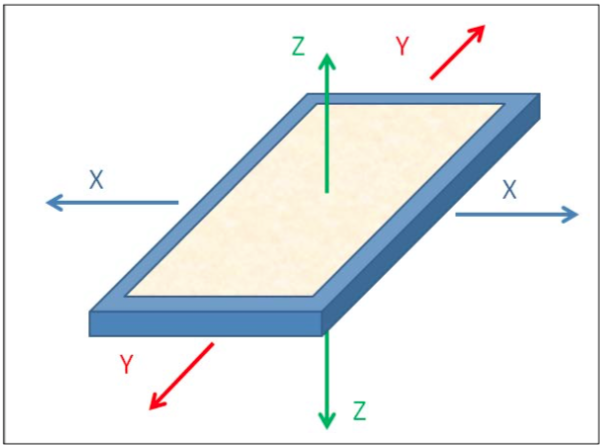
\includegraphics[width=15cm]{img/ejes.png}

	
	\clearpage

	\section{APIs}

	\clearpage

	\section{Realidad aumentada}



\end{document}









